\subsection{Cartes \emph{Arduino Mega}}

Le deuxième type de cartes que nous devions utiliser était l’\emph{Arduino Mega} 2560 (\cref{arduino}).
Les cartes \emph{Arduino} sont accompagnées d’un environnement de développement intégré spécifique, qui s’occupe de la compilation, l’installation et le suivi (console et autre outils intégrés).

\begin{figure}[H]
\centering
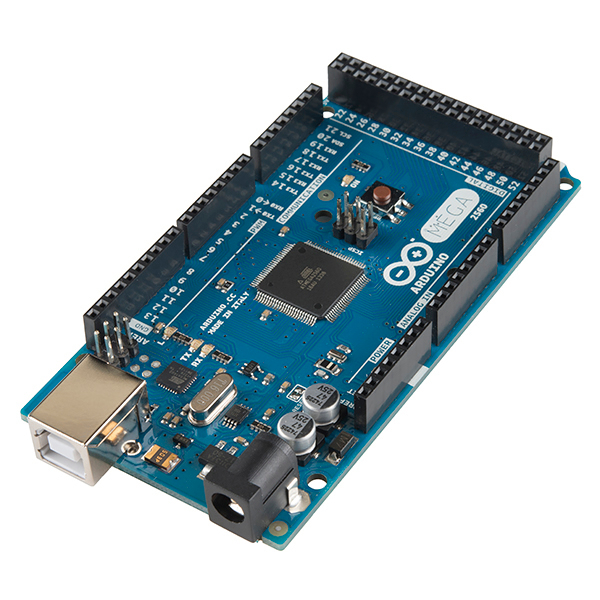
\includegraphics[width=8cm]{\rpDossier/images/arduino.jpg}
\caption{Carte \emph{Arduino Mega}}
\label{arduino}
\end{figure}

La communication sans fil n’est pas intégrée à cette carte \emph{Arduino}, contrairement à la CC 2538, aussi avons-nous utilisé une puce \emph{XBee} (\cref{xbee}), ainsi qu’une carte d’adaptation (à droite de la \cref{xbee-shields}).

\begin{figure}[H]
\centering
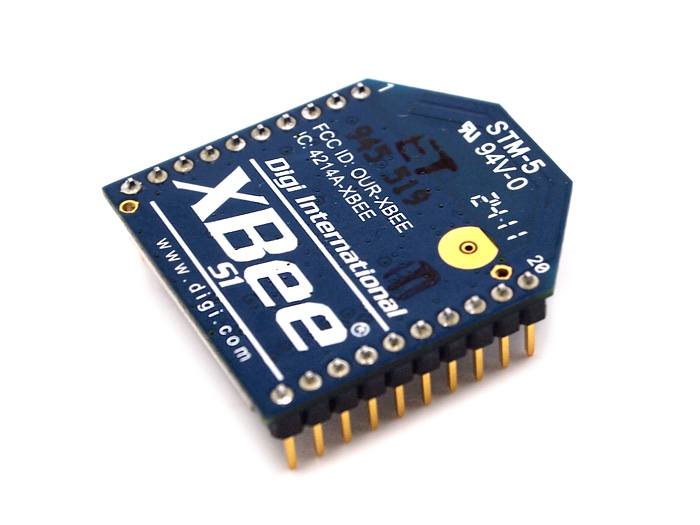
\includegraphics[width=5cm]{\rpDossier/images/xbee.jpg}
\caption{Puce \emph{XBee}}
\label{xbee}
\end{figure}

La carte d’adaptation que nous avons utilisée n’est pas la même que celle utilisée dans l’étude que nous devions reproduire \cite{eymery}, produite par \emph{Arduino} (à gauche de la \cref{xbee-shields}).
La plupart des documentations trouvées se référant à la carte d’Arduino, nous avons eu du mal à repartir de la documentation particulière de cette carte \citeweb{xbee-shield} pour simplement établir la communication entre la carte \emph{Arduino} et la puce \emph{XBee}. La fin du projet étant proche, nous avons décidé avec notre tuteur de nous concentrer sur les CC 2538.

\begin{figure}[H]
\centering
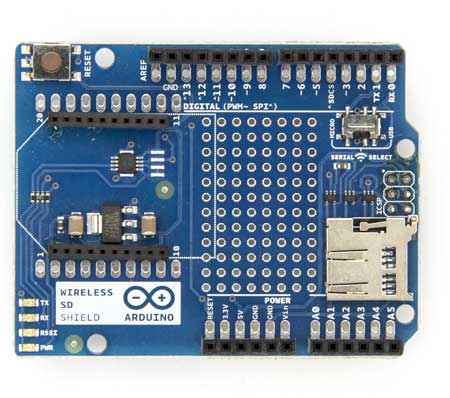
\includegraphics[height=6cm]{\rpDossier/images/arduino-shield.jpg}
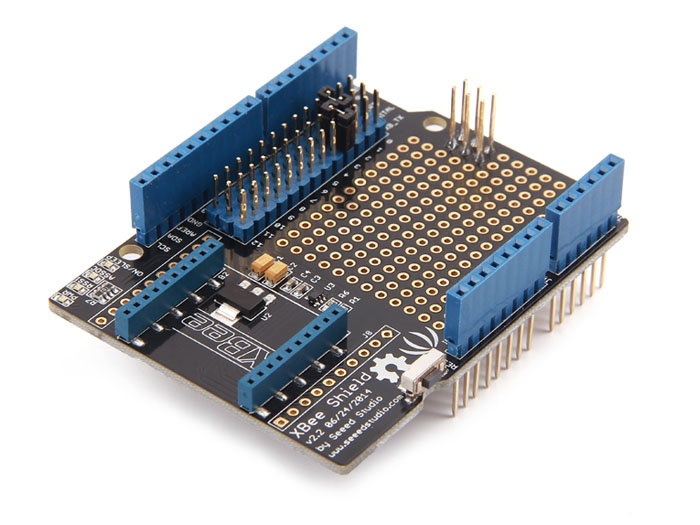
\includegraphics[height=6cm]{\rpDossier/images/xbee-shield.jpg}
\newline
À gauche la carte d’\emph{Arduino}, à droite celle de \emph{Seeed Studio}.
\caption{Cartes d’adaptation pour puce \emph{XBee}}
\label{xbee-shields}
\end{figure}
